\section{Methodology}
\label{sec:methodology}
We test whether using neutral-atom error probabilities changes the stabilizer
codes found by satisfiability-based code design. The calculation has three
stages: deriving a channel for a Rydberg pair, extracting its Pauli weights,
and selecting codes using different assumptions about the noise. Every code
is ultimately evaluated on the same target noise distribution.

\subsection{Rydberg channel and Pauli errors}
\label{sec:method_channel}
We model two atoms with local states
$\{|0\rangle,|1\rangle,|r\rangle,|L\rangle\}$.
The last state collects decay outside the computational and Rydberg levels;
it need not represent the physical loss of an atom from its trap.
The Rydberg-only pulse (hyperfine drive off) is governed by the coherent
Hamiltonian of Eq.~\eqref{eq:rydberg_three_level} and the master equation
\begin{equation}
\dot\rho=-\frac{i}{\hbar}[H(t),\rho]+
\sum_j\left(C_j\rho C_j^\dagger-
\tfrac12\{C_j^\dagger C_j,\rho\}\right).
\label{eq:res_lindblad}
\end{equation}
The collapse operators include Rydberg-state decay with branches
$(r\!\to\!0,r\!\to\!1,r\!\to\!L)=(0.053,0.053,0.894)$
and effective intermediate-state scattering with branches
$(e\!\to\!0,e\!\to\!1,e\!\to\!L)=(0.1354,0.2504,0.6142)$.
We use the 88~$\mu$s Rydberg and 110~ns intermediate-state lifetimes
reported in the experimental model, along with Gaussian quasi-static
detuning fluctuations on a $T_2^*=3~\mu$s coherence scale.
Treating these fluctuations as common to both atoms, and eliminating
the intermediate state, are explicit modeling approximations.

The complete channel maps a four-dimensional computational input to a
16-dimensional physical output. Let $M_j$ be its Kraus operators after
projection back to the computational subspace and removal of the chosen
noiseless reference evolution. The two-qubit Pauli-twirled weights are
\begin{equation}
q_P=\frac1{16}\sum_j
|\operatorname{Tr}(P^\dagger M_j)|^2,\quad
P\in\{I,X,Y,Z\}^{\otimes2}.
\label{eq:res_pauli}
\end{equation}
They need not sum to one because the projected channel loses probability
to the Rydberg and loss states. Such outcomes are recorded separately.
Pauli twirling also removes coherent terms present in the full channel.

\subsection{Stabilizer search and decoding}
For $n$ physical qubits and $r$ independent commuting stabilizers,
$k=n-r$ logical qubits are encoded. We use binary symplectic variables
for unrestricted $I,X,Y,Z$ generators and enforce commutation,
independence, and code distance. For exact correction of an error set
$\mathcal F$, every $E_a^\dagger E_b$, with $E_a,E_b\in\mathcal F$, must
either belong to the stabilizer group or anticommute with some generator.
These are Boolean SAT/SMT feasibility constraints.

For an independently checkable numerical optimum we enumerate all
commuting stabilizer groups for $n=4$, vary $k$, and require $d\geq2$.
SAT/SMT establishes feasibility; \emph{exhaustive evaluation}, rather than
a scalable weighted MaxSAT algorithm, selects the probability-optimal code.
The exact maximum-likelihood Pauli decoder chooses the most probable
stabilizer-equivalent error class for each syndrome:
\begin{equation}
p_{\mathrm{block}|\mathrm{comp}}
=1-\frac{\displaystyle\sum_s\max_L\sum_{E\in(s,L)}q_E}
{\displaystyle p_{\mathrm{comp}}},
\qquad p_{\mathrm{comp}}=\sum_Eq_E.
\label{eq:res_ml}
\end{equation}
Here block failure means an error in at least one of the encoded logical
qubits. Results are conditional on the final state remaining computational,
not circuit-level logical error rates.

To evaluate four physical qubits, we assume identical \emph{independent}
pair channels on atoms $(1,2)$ and $(3,4)$:
$q_{P_1P_2P_3P_4}=q_{P_1P_2}q_{P_3P_4}$.
This is a specified extension of a two-atom model, not a measured four-atom
channel. Codes are chosen under three alternative models: (i) uniform
single-qubit Pauli noise; (ii) single-qubit noise with the bias extracted
from the Rydberg channel; or (iii) the complete two-qubit Pauli weights.
All designs are finally tested under the same target noise.

\subsection{Experimental noise bias}
From the two-qubit Pauli distribution, define the first-qubit marginals
$p_A=\sum_{B\in\{I,X,Y,Z\}}q_{AB}$ for $A=X,Y,Z$.
The two atoms give equal values to numerical precision. We use
$\eta=p_Z/p_X$ and the observed approximate equality $p_Y=p_X$.
For the simpler independent-qubit comparison,
\begin{equation}
p_X=p_Y=\frac{p}{2+\eta},\quad
p_Z=\frac{\eta p}{2+\eta},\quad p_I=1-p
\label{eq:res_bias}
\end{equation}
with the \emph{same} $p=p_X+p_Y+p_Z$ in both cases.
We compare only $\eta=1$ and the derived $\eta_{\mathrm{hw}}$, rather
than fitting or sweeping an arbitrary physical bias.

\section{Results}
\label{sec:results}
\subsection{Extracted Rydberg error weights}
Table~\ref{tab:res_channel} shows the input-averaged output weights for
one two-atom pulse. The identity weight is large, but it is the identity
component of the \emph{Pauli-twirled} channel, not a direct experimental
count of error-free gates.

\begin{table}[t]
\caption{Output weights of the reduced two-atom Rydberg channel.
The first two rows refer to computational Pauli outputs.}
\label{tab:res_channel}
\begin{ruledtabular}
\begin{tabular}{lr}
Outcome & Probability (\%)\\
\hline
Identity ($II$) & 99.757083\\
Other Pauli strings & 0.089403\\
Residual Rydberg excitation & 0.028215\\
At least one atom in $|L\rangle$ & 0.125299\\
\hline
Total & $\simeq100$\\
\end{tabular}
\end{ruledtabular}
\end{table}

The leading nonidentity terms are $q_{ZI}\simeq q_{IZ}
=2.7693\times10^{-4}$ and $q_{ZZ}=2.5053\times10^{-4}$.
The effective single-qubit marginals are
\begin{align}
p_X&=p_Y=2.24149\times10^{-5},\nonumber\\
p_Z&=5.49852\times10^{-4},\qquad
\eta_{\mathrm{hw}}=24.5307.
\label{eq:res_eta}
\end{align}
The bias follows from the saved channel results, not from an adjustable
noise parameter. Correlated $ZZ$ errors and loss remain outside the
independent single-qubit description.

\subsection{Varying the number of logical qubits}
With four physical qubits and $d\geq2$, exhaustive enumeration finds
2268 stabilizer groups with $k=1$ and 216 with $k=2$.
No $[[4,3,d\geq2]]$ code exists. Under the full two-pair Rydberg
Pauli model, the respective best \emph{conditional} block-error
probabilities are $0.037867\%$ for $[[4,1,2]]$ and
$0.095871\%$ for $[[4,2,2]]$. Encoding twice as many logical qubits
therefore raises the block-error probability. Neither point dominates
the other in rate and reliability; this is a finite-size Pareto
comparison, not a general claim about larger codes.

\subsection{Uniform versus hardware-bias-informed design}
For the independent-qubit experiment we fix the marginal error strength
$p=5.94682\times10^{-4}$ obtained above and use
$\eta\in\{1,24.5307\}$. All candidate codes have $d\geq2$ and
\emph{no Hamiltonian seed}. At $\eta=1$, both search methods coincide:
the optimal block-error probabilities are $0.118897\%$ ($k=1$) and
$0.178298\%$ ($k=2$). At $\eta_{\mathrm{hw}}$, the results are given
in Table~\ref{tab:res_bias} and Fig.~\ref{fig:res_bias}.

\begin{table}[t]
\caption{Conditional block error (\%) under the same independent Pauli
channel with $\eta=24.5307$. The uniform-design column is the
\emph{median} over its equally optimal codes.}
\label{tab:res_bias}
\begin{ruledtabular}
\begin{tabular}{lrrr}
Code & Uniform design & Bias-informed & Reduction\\
\hline
$[[4,1,2]]$ & 0.066190 & 0.013544 & 79.5\%\\
$[[4,2,2]]$ & 0.125649 & 0.072999 & 41.9\%\\
\end{tabular}
\end{ruledtabular}
\end{table}

\begin{figure}[t]
\centering
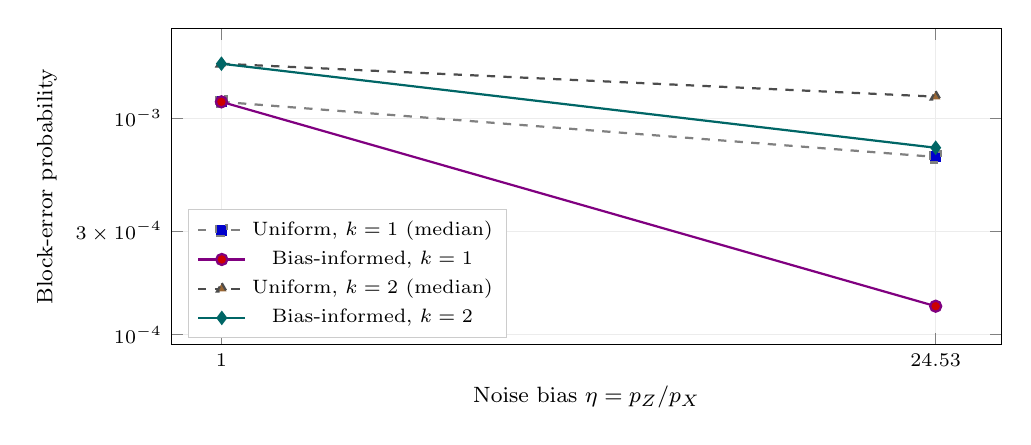
\begin{tikzpicture}
\begin{loglogaxis}[
width=\columnwidth,height=5.6cm,
xmin=0.8,xmax=33,ymin=0.00009,ymax=0.0026,
xtick={1,24.5306954},xticklabels={$1$,$24.53$},
ytick={0.0001,0.0003,0.001},
yticklabels={$10^{-4}$,$3\times10^{-4}$,$10^{-3}$},
xlabel={Noise bias $\eta=p_Z/p_X$},
ylabel={Block-error probability},
grid=both,grid style={gray!15},
legend style={font=\scriptsize,at={(0.02,0.02)},anchor=south west,
fill=white,draw=gray!40},
tick label style={font=\scriptsize},label style={font=\footnotesize}]
\addplot+[gray,dashed,thick,mark=square*] coordinates
{(1,0.0011889703697) (24.5306954,0.0006618975869)};
\addlegendentry{Uniform, $k=1$ (median)}
\addplot+[violet,thick,mark=*] coordinates
{(1,0.0011889703697) (24.5306954,0.0001354364468)};
\addlegendentry{Bias-informed, $k=1$}
\addplot+[black!70,dashed,thick,mark=triangle*] coordinates
{(1,0.0017829843998) (24.5306954,0.0012564876793)};
\addlegendentry{Uniform, $k=2$ (median)}
\addplot+[teal!80!black,thick,mark=diamond*] coordinates
{(1,0.0017829843998) (24.5306954,0.0007299909488)};
\addlegendentry{Bias-informed, $k=2$}
\end{loglogaxis}
\end{tikzpicture}
\caption{Exact two-point comparison of uniform and hardware-bias-informed
design. The physical single-qubit error strength is fixed while the bias
changes. The uniform curves show medians across tied optimal codes.
Connecting segments guide the eye; they are not a sweep of experimental
parameters. Independent noise and computational outputs are assumed.}
\label{fig:res_bias}
\end{figure}

To check whether the simple bias approximation captures the full model,
we also evaluate selected codes using \emph{all 256} Pauli weights obtained
from the two independent Rydberg pairs (Table~\ref{tab:res_full}).
The uniform entries are illustrative choices among tied uniform-optimal
codes; the table must not be read as a guaranteed improvement over every
possible uniform-noise solution. For $k=1$, 64 of the 324 codes tied under
uniform two-qubit Pauli noise also attain the full-hardware optimum.

\begin{table}[t]
\caption{Conditional block error (\%), all codes tested under the
same full two-pair Rydberg Pauli model.}
\label{tab:res_full}
\begin{ruledtabular}
\begin{tabular}{lrrr}
Code & Uniform example & Bias-informed & Full-informed\\
\hline
$[[4,1,2]]$ & 0.116812 & 0.038589 & 0.037867\\
$[[4,2,2]]$ & 0.149033 & 0.095871 & 0.095871\\
\end{tabular}
\end{ruledtabular}
\end{table}
The two-pair computational survival is $99.693208\%$; the
out-of-computational outcomes are not corrected by this Pauli decoder.

\subsection{Hamiltonian seeds}
For the Rydberg-only Hamiltonian, the single-atom operator
$Q=|0\rangle\langle0|-|1\rangle\langle1|-|r\rangle\langle r|$
commutes with the coherent drive. Its restriction to computational
states is $Z$, motivating the seed $ZZII$.
The symmetry need not survive a hyperfine drive or dissipative jumps;
requiring a seed does not make the entire code invariant under open-system
evolution. For $[[4,1,2]]$, the seeded and unseeded conditional errors
are $0.037868\%$ and $0.037867\%$, respectively, so the seed gives no
meaningful improvement. For $k=2$ there is no distance-two four-qubit
code containing this seed. Hamiltonian-seeded searches can therefore
exclude useful codes as well as guide code selection.

\section{Discussion}
\label{sec:discussion}
The main result is that physical noise information can resolve code
choices that a uniform model cannot distinguish. In the independent
bias comparison, the bias-informed code improves over the median
uniform-optimal design by $79.5\%$ for $k=1$ and $41.9\%$ for $k=2$.
However, many uniform-noise optima are tied, and some also perform
optimally under the hardware noise. The defensible conclusion is that
the physical probabilities provide a principled basis for \emph{selecting}
among those codes, not that they reveal codes inaccessible to SAT.

The present search covers only a four-qubit budget, and the best
distance-two code does not generally correct every single-qubit Pauli
error. The solver uses SAT/SMT for stabilizer feasibility followed by
exhaustive probability ranking, not yet scalable weighted MaxSAT.
Furthermore, the Rydberg channel is an approximate physical simulation,
not measured process tomography. The assumed detuning correlation,
effective intermediate-level elimination, and independent four-atom
extension require further validation. Leakage and residual Rydberg
population are not included in the reported conditional logical errors.
Thus these data should not be identified with measured fault-tolerant
QEC performance or a pseudothreshold.

\section{Conclusion and Future Outlook}
\label{sec:conclusion}
We constructed a physically motivated two-atom Rydberg noise model and
used its error probabilities to compare stabilizer-code selection.
Allowing $k$ to vary exposes a rate--reliability trade-off, and
hardware-bias information can improve code selection relative to typical
uniform-noise choices. Constraining stabilizers with an available
Hamiltonian symmetry did not improve this small-system optimum.
Future work requires larger $[[n,k,d]]$ searches, uncertainty studies
of the physical parameters, loss-aware decoding, and repeated
syndrome-extraction circuits before claims about scalable hardware-aware
error correction can be made.
